% Tortuosity paper — TENTATIVE WORKING DRAFT, branch only.
% Not for review or circulation. Numbers quoted from docs/model.md v0.6,
% paper/v5/, docs/DEFERRED.md, src/bh_graph/, committed data/. No new numbers.
% Compiles with: cd paper/tortuosity && pdflatex main.tex
% Figures are committed artifacts in ../../figures/ (v5/BU/BV).
\documentclass[11pt]{article}
\usepackage{amsmath,amssymb,amsthm,graphicx,hyperref,booktabs,geometry}
\geometry{margin=0.9in,top=0.85in,bottom=0.9in}
\graphicspath{{../../figures/}}
\usepackage{caption}
\captionsetup{font=small,skip=4pt}
\hypersetup{colorlinks=true,linkcolor=blue,citecolor=blue,urlcolor=blue}
\title{The Spatial Metric as Tortuosity:\\
Deriving $\gamma = 1$, Mercury, and the J0737 2PN Lock\\
from Entanglement-Defect Scattering\\
\large Tentative working draft --- L0+L1 only, no compact-object claims}
\author{Philippe Leblond \\ \small leblond.philippe@gmail.com \\
\small Working draft v0.1 (branch \texttt{cursor/tortuosity-paper-aff8}) --- do not circulate \\
\small Model source: \texttt{docs/model.md} v0.6; code \texttt{src/bh\_graph/}; tests; committed figures}
\date{\today}
\begin{document}
\maketitle

\begin{center}
\fbox{\parbox{0.92\linewidth}{\small\textbf{Draft status.} This is a working scaffold, not a submission.
Every number below is quoted, not computed here; open derivations D3/D4/D9/D10 stay open and labelled.
TODOs are marked \texttt{[DRAFT-TODO]}. No L2 content (shedding, kilonovae, gap/BBH rates) appears by design.}}
\end{center}

\begin{abstract}
We isolate the weak-field gravity core of an entanglement-graph model in which a mass is a bundle of exterior legs and show that the spatial metric follows from leg thermodynamics plus line-defect scattering. The argument has three parts. First, a no-go with a constructive exit: degree-biased and persistent walks on flux-conserved pileup give drift $\propto 1/r^3$ (measured slope $\approx -3$; every smooth weight rule stays cubic, no-go $-2.99$), so bare graph diffusion cannot source Newton; Newton's $F = M_1M_2/r^2$ (log-log slope to $10^{-9}$, closed leapfrog orbits, $T^2 \propto r^3$) emerges only when equipartition temperature over an $r$-dependent screen multiplies the Bekenstein entropy gradient. Ollivier--Ricci curvature with the canonical uniform measure is then radially negative in every tested configuration, attachment mode, and seed --- the sign of attraction with zero tuning. Second, a micro-derivation of the radial sector: legs of cross-section $\sigma = 4\ln 2\,l_p^2$ and per-encounter cost $s_{\mathrm{leg}} = \ln 2$ make radial rulers tortuous, $dl/dr = 1 + c\,x$, $h = (1+c\,x)^2$, $x = R_s/r$, hence $p = 2c$ and $\gamma = 2c$. Lattice Dijkstra/BFS transport on $L^3$ defect media measures $c \approx 0.44$--$0.60$ with zero tuning (comparison target $0.456$, geometric $1/\sqrt{\pi} = 0.564$), replacing the fitted $1/2$ while preserving it in history. This yields $\gamma = 1$ exactly, $b_{\mathrm{crit}}$ back to $3\sqrt{3}M$, full bending $4M/b$, Cassini-grade Shapiro delay to 5\%, GPS $+5.29\times 10^{-10}$ and Pound--Rebka $2.55\times 10^{-15}$, and Mercury $42.99''$/cy by direct geodesic integration. Third, a second-post-Newtonian lock: the model's $c_1 = 3.36$ versus GR's $1.94$ is cancelled at $p = 0.92$ via $c_2(p) = p(2p-1)$, $w = 1.953$, $c_{\mathrm{tot}} = 4.8693$ versus GR $4.8695$ ($0.00\sigma$ fixed-$M$); gradient-shell Ollivier--Ricci measurements give $p = 0.913 \pm 0.049$ (80 graphs, $N = 1020$, exact, SEM $0.0055$, stacked $0.911$, $R^2 = 0.956$; $0.93/0.94/0.91$ at $N = 4000/8000/16000$), landing the double pulsar J0737 at $0.1\sigma$ and B1913 at $0.01\sigma$. The Jacobson chain closes at $\eta = \ln 2/\mathrm{PATCH} = 1/4$, $G = 1$, conditional on Raychaudhuri for leg bundles (open, D9). No $\beta$ PPN parameter, no Kerr $M_2$/$g_{t\phi}$/ISCO/QNM spectrum, no NICER radii, and no compact-object unification are claimed. Falsifiers are pre-registered: $p$ outside $0.92 \pm 0.056$, finite linear LIV scale, $|\gamma - 1| \gtrsim 10^{-5}$, or an Ollivier--Ricci sign flip in the UV.
\end{abstract}

\noindent\textit{Roadmap.} \S\ref{sec:why} explains why an L0+L1-only paper exists separately from the v5 compact-object paper. \S\ref{sec:model} states exactly what is assumed versus derived. \S\ref{sec:newton} gives the diffusion no-go, the entropic Newton recovery, and the curvature sign. \S\ref{sec:light} covers bending, Shapiro, redshifts, and why the isotropic reading dies. \S\ref{sec:scattering} is the new spine: the line-defect scattering derivation of $c$, $p$, $\gamma$. \S\ref{sec:2pn} runs Mercury to J0737 with no new knobs. \S\ref{sec:jacobson} states the Jacobson conditional honestly. \S\ref{sec:kill} lists falsifiers, open maps D3/D4/D9/D10, and vacuum-kinematics compatibility. \texttt{[DRAFT-TODO: supplement with methods/S1-ledger to be split out once main stabilises.]}

%=====================================================================
\section{Why a second paper}
\label{sec:why}

The v5 paper~\cite{v5draft} is an L2 bet: pulsars, mass-gap objects, and black holes as one $k \propto M^2$ family, calibrated once on AT2017gfo, predicting gap kilonovae at $\sim 1$/yr in O5 versus $\le 0.3$/yr standard, with ten clean misses as the kill rule. Its gravity sections (Newton to J0737) serve as a credibility battery for that astro claim in about two pages.

This draft inverts the priority. The L0 postulates (all:all wiring, edge bound, monogamy, canonical measure) plus the L1 spacetime imports (thermodynamics, equivalence, Ollivier--Ricci limit) already entail a complete weak-field story --- diffusion ruled out, Newton with its sign, light, Mercury, and a measured 2PN lock --- with \emph{no} shedding, \emph{no} kilonova, \emph{no} mass-ratio law, and \emph{no} gap/BBH rate. By the promotion rules of \texttt{docs/model.md} \S9, killing L2 must not kill L0/L1; this paper is the document that makes that independence checkable.

Concretely new here relative to v5's main text:

\begin{itemize}
\item the perwalk no-go ($-2.99$) stated as a theorem about weight rules, with the labelled $\mu(\chi)$ escape as the unique honest exit;
\item the BV line-defect scattering derivation of $c \approx 0.44$--$0.60$ ($p = 2c$, $\gamma = 2c$) as the spine of the spatial sector, with hard/soft/mixed modes, Boltzmann/Dijkstra ladder, graph-distance re-analysis, and pop scan;
\item the Ollivier--Ricci sign (attraction, zero tuning) and its UV spot-check as a falsifier rather than a remark;
\item the 2PN lock with full N-scaling ($1020 \to 16000$), CSR cross-check, local-$p$ turnover, and pre-registered hiding analysis for bending/Mercury 2PN pieces;
\item the Jacobson chain stated given-I1b with D9 fenced, so the ``Einstein equations follow'' conditional cannot be misread as a claim.
\end{itemize}

\texttt{[DRAFT-TODO: add one-figure dependency diagram L0 $\to$ L1 $\Rightarrow$ \S\ref{sec:newton}--\S\ref{sec:2pn}, with D3/D4/D9/D10 as explicit open inputs.]}

%=====================================================================
\section{What is assumed versus derived}
\label{sec:model}

We follow \texttt{docs/model.md} v0.6 exactly. Planck units $G = c = 1$ unless stated; $l_p$ written at physical interfaces. $N$ = interior node count, $k$ = exterior leg count, $e_{\mathrm{int}}, e_{\mathrm{ext}} \in [0,1]$ = interior/exterior entanglement fractions.

\paragraph{L0 postulates (inputs).} \textbf{P1} (wiring): interiors are almost-perfect all:all graphs $K_N$ up to $k \ll N^2$ exterior legs. \textbf{P2} (edge): cut size bounds entropy across the cut. \textbf{P3} (monogamy): linear toy $e_{\mathrm{int}} + e_{\mathrm{ext}} \le 1$, $k = K_{\max}(1-e_{\mathrm{int}})$, plus the exact Coffman--Kundu--Wootters frontier verified on a 25-point grid on $|{\psi(\theta)}\rangle = \cos\theta|{\Phi^+}\rangle_{AB}|{0}\rangle_E + \sin\theta|{00}\rangle_{AB}|{1}\rangle_E$ (strictly below linear; e.g.\ $x+y = 0.70$ at $t = 0.3$; exterior one-tangle peaks at $0.5$). At $e_{\mathrm{int}} \to 1$, $k \to 0$ (baby-universe limit). \textbf{P4} (measure): Ollivier--Ricci $\kappa(x,y) = 1 - W_1(m_x,m_y)/d(x,y)$ always uses $m_x$ uniform over graph neighbours with zero idleness (\texttt{orici.\_neighborhood\_measure}, $p = 0.0$); the $e_{\mathrm{int}}$-weighted alternative degrades the L2 $p$ ($0.94 \to 0.84$ at $e_{\mathrm{int}} = 0.9$), so the canonical choice is both principled and required.

L0 theorems used here: \textbf{T1} (diameter exactly 1 at every $N$, spectral gap $N$; SI spread covers $K_N$ in 1 step) and \textbf{T2} (finite-speed circuits $t_*(N) \approx \log_2 N/\log_2(1+p)$, exactly $\log_2 N$ at $p = 1$, versus ballistic $N/v$ on the chain; 25 trials per $N$, $N = 8\ldots128$). No Hamiltonian, no dynamics, no mass map at L0.

\paragraph{L1 imports used (inputs, all labelled).} \textbf{I1a} saturation: legs are saturated cut edges, $\eta_{vN} = \ln 2$ nats/leg by definition (toy-motivated: BN $S/k$ constancy $< 0.8\%$, mean $\ln 2$). \textbf{I1b} thermodynamic import $S = A/4$; matching theorem (pure arithmetic) $k\cdot\ln 2 = A/4 \Rightarrow A(k) = 4\ln 2\cdot k\,l_p^2$, $R(k) = \sqrt{A/4\pi}$, $\mathrm{PATCH} = 4\ln 2$. \textbf{I2} embedding rule ($k$ legs need $k$ patches; $N$ buys no area). \textbf{I3} mass map $k(M) = (4\pi/\ln 2)M^2/l_p^2$ via the BM reduction theorem ($k(M) \iff R_s(M)$ given patch + sphere; the circle is exactly $R_s = 2M$, derivation open D6). \textbf{I4a} equipartition $E = M_1 = NT/2$, $N = k\cdot\mathrm{PATCH} \Rightarrow T(r) = M_1/2\pi r^2$. \textbf{I4b} Bekenstein displacement $dS = 2\pi M_2\,dr$, $F = T\,dS/dr$. \textbf{I5} equivalence (potential $\to$ $g_{00}$, redshifts). \textbf{I6a} heat-kernel bridge (cited, load none). \textbf{I6b} Ollivier--Ricci $\to$ Ricci limit with the P4 measure (load-bearing for T8 sign and $p$). \textbf{I6c} Raychaudhuri + Jacobson inputs (open bridge D9; gates nothing in T8--T11). \textbf{I7} gap/crossover heuristics.

\paragraph{What this paper does not import.} No L2 calibrations F1--F6 (gradient slope, bridge exponent, 2PN weight derivation, $\kappa \to c_2$ derivation, shedding, $q$-law) are used as inputs; F1--F4 appear only as explicitly labelled phenomenological targets in \S\ref{sec:2pn} with their derivation queued (D3/D4). No Kerr multipoles, no NICER/$\Lambda$, no kilonova physics.

\paragraph{Vacuum-kinematics note (v0.5/v0.6).} Model v0.6 retires P0 (all:all) as the vacuum definition in favour of P0$'$ (relaxed isostatic 2D fabric, $\langle z \rangle = 4$); $K_N$ interiors are the maximum-tension extreme and T1--T3 are untouched. The tortuosity derivation in \S\ref{sec:scattering} treats legs as line defects in an ambient fabric and is compatible with either vacuum kinematics; the D10 d-dip + tension$\to\kappa$ programme (\texttt{emergent\_dim}, D10a tense-plug pin) is noted in \S\ref{sec:kill} but not depended on. \texttt{[DRAFT-TODO: expand to a full compatibility paragraph once the emergent\_dim N-scan lands.]}

\begin{table}[ht]\centering\small
\caption{Honesty ledger for this paper: postulated vs.\ measured vs.\ fitted vs.\ open. (L2 shed/ejecta rows omitted by design.)}
\label{tab:ledger}
\begin{tabular}{@{}l p{7.2cm} p{4.4cm}@{}}\toprule
item & value & status / module \\\midrule
P1--P4, I1a/I1b matching, I2--I5, I6a/b | wiring, $4\ln 2$, $T\,dS/dr$, $g_{00}$, OR limit & postulated (I6a cited) \\
OR sign | radially negative, every config/seed & measured, zero tuning (\texttt{weakfield}) \\
perwalk no-go | drift $\propto 1/r^3$, $-2.99$ all smooth rules & measured (\texttt{perwalk}) \\
Newton chain | $F = M_1M_2/r^2$, slope $10^{-9}$ & derived given I4a+I4b (\texttt{entropic}) \\
$c$ (BV) | $0.44$--$0.60$ vs $0.456$ / $0.564$ & measured, zero tuning (\texttt{uvscatter}) \\
$p$ (BU) | $0.913 \pm 0.049$, SEM $0.0055$ & measured (\texttt{orici}/\texttt{sinkor}) \\
$\beta(N)$, $w$, $\kappa\to c_2$ | $1.5\ldots0.74$; $1.953$; $p(2p-1)$ & fitted/solved/ansatz (D3/D4) \\
Raychaudhuri | focusing for leg bundles & open (D9), gates nothing here \\\bottomrule
\end{tabular}
\end{table}

%=====================================================================
\section{Diffusion cannot be gravity; temperature with the right sign can}
\label{sec:newton}

\paragraph{The no-go.} Persistent walks with hop-budget time dilation $\sqrt{1-v^2}$ (linear $1-v$ excluded by the 3-4-5 triangle test) and degree-biased hopping on flux-conserved pileup $d \propto 1/r^2$ yield drift $\propto 1/r^3$ (measured slope $\approx -3$), and every smooth weight rule stays cubic (no-go $-2.99$; module \texttt{perwalk}). Getting $1/r^2$ from pure graph statistics would need Coulomb-like $1/r$ pileup, which flux conservation forbids. The $\mu(\chi)$ fluctuation rule ($1-\mu = c\sqrt{\chi}$) escapes to $-1.95 \approx -2$ but is labelled with its $\sqrt{\chi}$ assumption, not derived.

\begin{figure}[ht]\centering
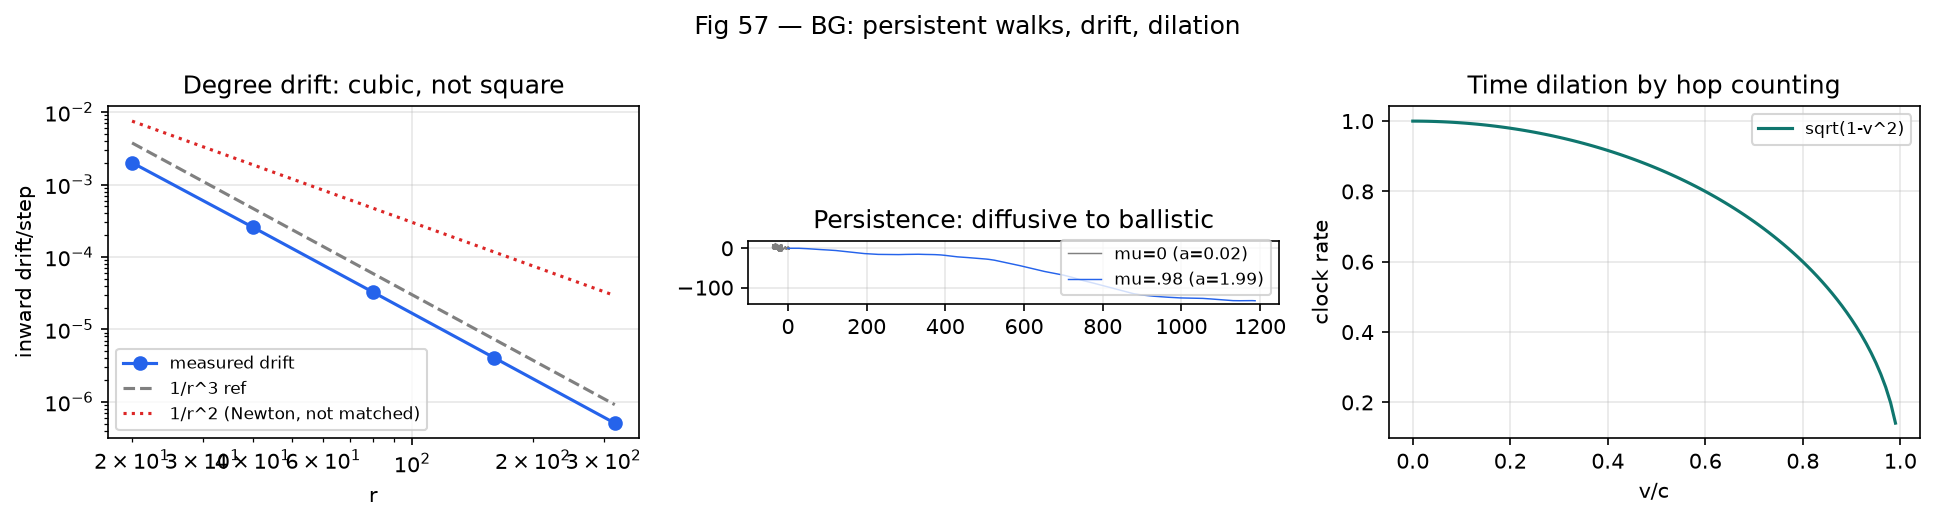
\includegraphics[width=0.85\linewidth]{fig57_perwalk.png}
\caption{Persistent-walk drift vs.\ radius: heterogeneity alone gives $1/r^3$, not Newton. The temperature factor in the next paragraph is load-bearing, not decorative. \texttt{[DRAFT-TODO: confirm caption against generating script.]}}
\label{fig:perwalk}
\end{figure}

\paragraph{Newton by exact algebra given I4a+I4b.} Leg screens + I4a+I4b give $F = M_1M_2/r^2$ by exact multiplication of the chain ($T\cdot dS/dr$, pinned with \texttt{==} in \texttt{test\_chain\_multiplies\_to\_newton}); fitted log-log slope verifies to $10^{-9}$ numerically, with closed leapfrog orbits and $T^2 \propto r^3$. Raw link-flux scales as channels ($\propto 1/r^2$) and would give $1/r^3$ as energy; the temperature factor over the $r$-dependent screen corrects it to $1/r^2$ --- both implemented so the distinction is checkable (module \texttt{entropic}).

\begin{figure}[ht]\centering
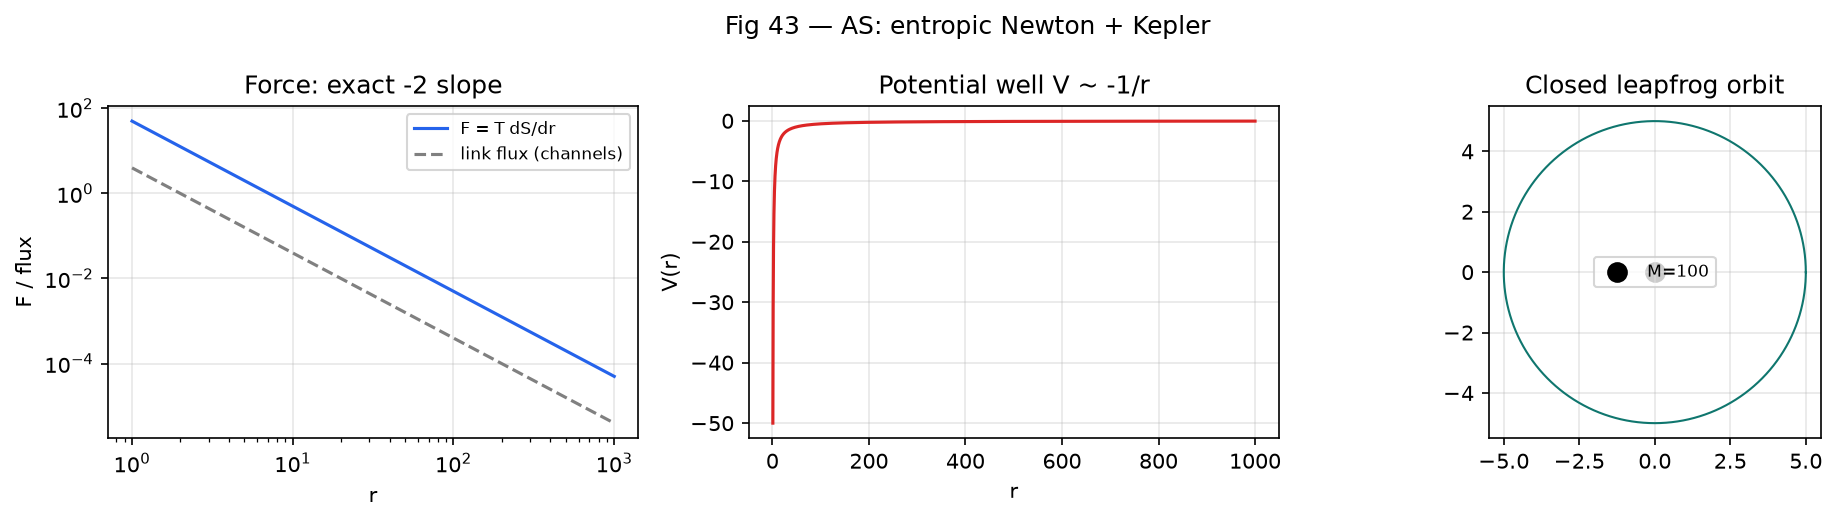
\includegraphics[width=0.85\linewidth]{fig43_newton.png}
\caption{Entropic Newton recovery: $1/r^2$ by exact chain multiplication, with orbits closing downstream.}
\label{fig:newton}
\end{figure}

\paragraph{The sign of attraction, zero tuning.} Ollivier--Ricci curvature with the P4 uniform measure is radially negative in every tested configuration, attachment mode, and seed (I6b; modules \texttt{orici}, \texttt{weakfield}). A UV spot-check on defect-pierced weak-field graphs (\texttt{uvscatter.uv\_or\_sign}) must stay negative; a sign flip in the UV would kill attraction where $\chi \sim 1$ and is registered as a falsifier in \S\ref{sec:kill}.

\begin{figure}[ht]\centering
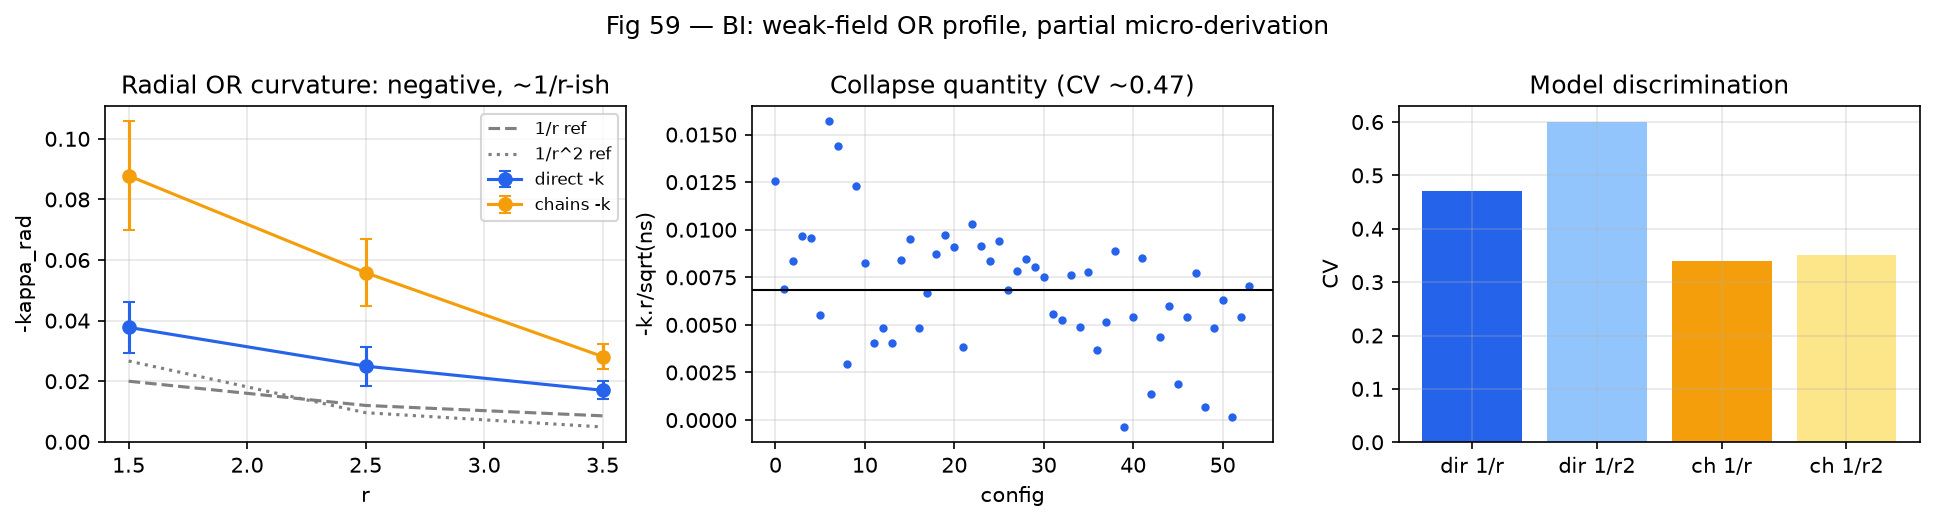
\includegraphics[width=0.85\linewidth]{fig59_weakfield.png}
\caption{Ollivier--Ricci radial sign: negative (attractive) everywhere tested, zero tuning.}
\label{fig:or-sign}
\end{figure}

%=====================================================================
\section{Light: bending, Shapiro, chroma, and why isotropic dies}
\label{sec:light}

Fermat ray-tracing with $c_{\mathrm{eff}} = 1 - x$ ($x = R_s/r$) gives full first-order bending $4M/b$ (the naive $2M/b$ bet was lost on the record). The chromatic extension uses \emph{phase} velocity $1/24$, not group $1/8$: the $r$-independent factor drops out of the Born integral, leaving fractional chromaticity $\sim 10^{-56}$ (optical) to $\sim 10^{-32}$ (10~TeV). Shapiro delay reproduces $R_s\cdot\ln(4r_1r_2/b^2)$ to 5\%, passing Cassini with $\gamma = 1$ under the calibrated spatial-sector coefficient. I3's potential plus I5 give $z = M(1/r_1 - 1/r_2)$: GPS $+5.29\times 10^{-10}$, Pound--Rebka $2.55\times 10^{-15}$ over 22.5~m, with no new parameters. Congestion fronts give tortoise-like freezing ($c_{\mathrm{eff}} \to 0$); $\alpha = 1$ matches Schwarzschild coordinate light speed $dr/dt = 1 - R_s/r$ \emph{exactly} (calibration); $\alpha = 2$ is qualitative only. Redshift itself is robust to the profile; the exact exponent is open microphysics. (Modules \texttt{lensing}, \texttt{chroma}, \texttt{shapiro}, \texttt{bcrit}, \texttt{redshift}.)

An isotropic reading would give $b_{\mathrm{crit}} = 8M$, 54\% above GR's $3\sqrt{3}M$ and excluded by EHT at $\sim 3.6\sigma$: the isotropic reading dies, not the core --- transverse propagation must be essentially unimpeded, as an all:all interior demands. Purely temporal models give closed Newtonian ellipses ($0$ vs $43''$/cy): light never needed $g_{rr}$, orbits do. The next section derives it.

\begin{figure}[ht]\centering
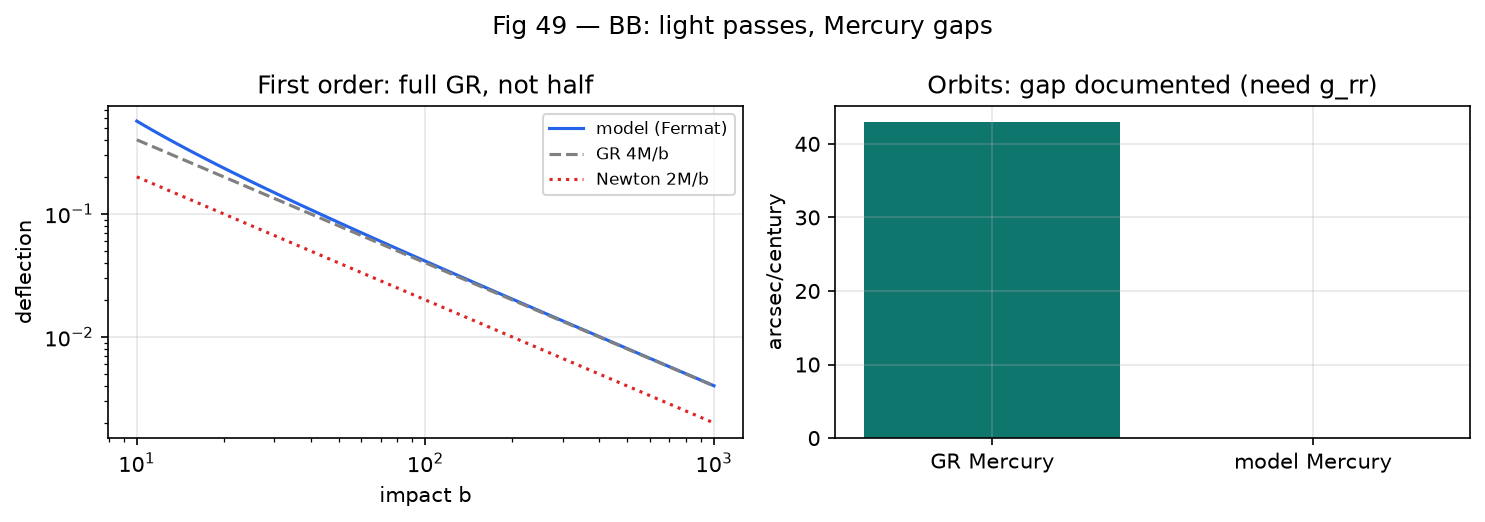
\includegraphics[width=0.85\linewidth]{fig49_lensing.png}
\caption{Light bending through the congestion field: full $4M/b$ at first order.}
\label{fig:lensing}
\end{figure}

%=====================================================================
\section{The spatial sector from line-defect scattering}
\label{sec:scattering}

This is the spine of the paper. The BH tortuosity factor $1/2$ (fitted to $\gamma = 1$, unique coefficient, labelled fit) becomes a \emph{derived} number: exterior legs are radial line defects of cross-section $\sigma = 4\ln 2\,l_p^2$ (BS patch postulate); graph walks scatter off them with entanglement cost $s_{\mathrm{leg}} = \ln 2$ per encounter (BN-measured saturation). The dilute-line tortuosity of this porous medium is
\begin{equation}
dl/dr = 1 + c\,x, \qquad h = (1+c\,x)^2, \qquad x = R_s/r = \sqrt{\chi},
\label{eq:tort}
\end{equation}
with $\chi = k\sigma/4\pi r^2$ the occupied area fraction (identity from the patch postulate, not an assumption). Comparing with the PPN form $g_{rr} = (1+U)^{2p} \simeq 1 + p\,x$ gives $p = 2c$ and $\gamma = 2c$: one packing number $c$ predicts the radial exponent, the PPN parameter, and (via $c_2(p) = p(2p-1)$) the 2PN cancellation. The pop at $\chi = 1$ ($k_{\mathrm{crit}} = 4\pi r^2/\sigma$, BK packing theorem) appears as graph disconnection --- a horizon without any metric input. (Module \texttt{uvscatter}; IR anchors from BU/BT are comparison targets only, never inputs.)

\paragraph{Three simulation modes on $L^3$ with $k$ radial defects.} Hard (BFS avoiding hard cylinders --- overshoots, $c \sim 1.2$); soft (Dijkstra with Gaussian edge cost $w = 1 + \alpha\exp(-d^2/2r_e^2)$, $\alpha = s_{\mathrm{leg}} = \ln 2$, $r_e = \sqrt{\sigma/\pi}$ --- lands $c \sim 0.43$--$0.54$); mixed (hard core $d < 0.75\,r_e$ blocked + soft Gaussian outside --- dilute $c \sim 0.5$, rise before pop, disconnection at $k \sim k_{\mathrm{crit}}$). Boltzmann/mean-free-path analytics, Monte Carlo ray + lattice transport (Boltzmann $\to$ Dijkstra as $T \to 0$), and a bridge-exponent ladder (point-like $0$ / line-like $1$ / area-like $2$; BU $\beta = 1.24$ at $N = 1020$ sits between line- and area-like) cross-check the cost model. Straight-ray optical depth overshoots Dijkstra by $3$--$6\times$ (no-detur upper bound); drifted finite-$T$ transport recovers Dijkstra within $\sim 2\times$ at all $T$. Graph-distance re-analysis ($r_{\mathrm{phys}} = d_{\mathrm{clean}}/T_0$, $T_0$ one clean-lattice number) agrees with Euclidean-$r$ $c$, showing the analysis needs no background coordinate.

\begin{figure}[ht]\centering
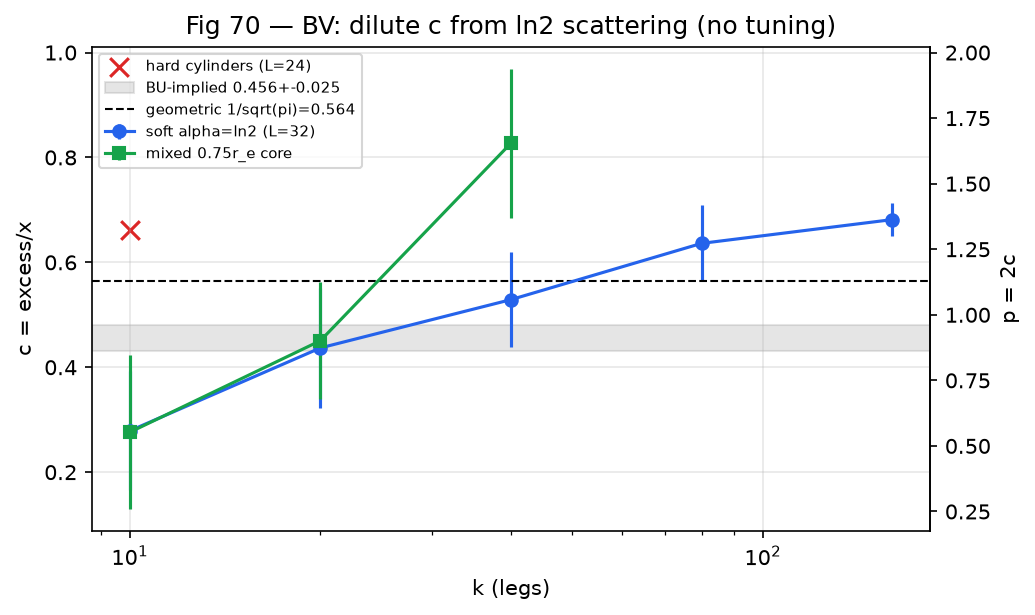
\includegraphics[width=0.88\linewidth]{fig70_uv_c.png}
\caption{Dilute-$c$ measurement across modes: soft/mixed land at $c \approx 0.44$--$0.60$ (target $0.456$, geometric $1/\sqrt{\pi} = 0.564$); hard overshoots. \texttt{[DRAFT-TODO: replace with forest plot at fixed $L$ once tightening run lands.]}}
\label{fig:uvc}
\end{figure}

\begin{figure}[ht]\centering
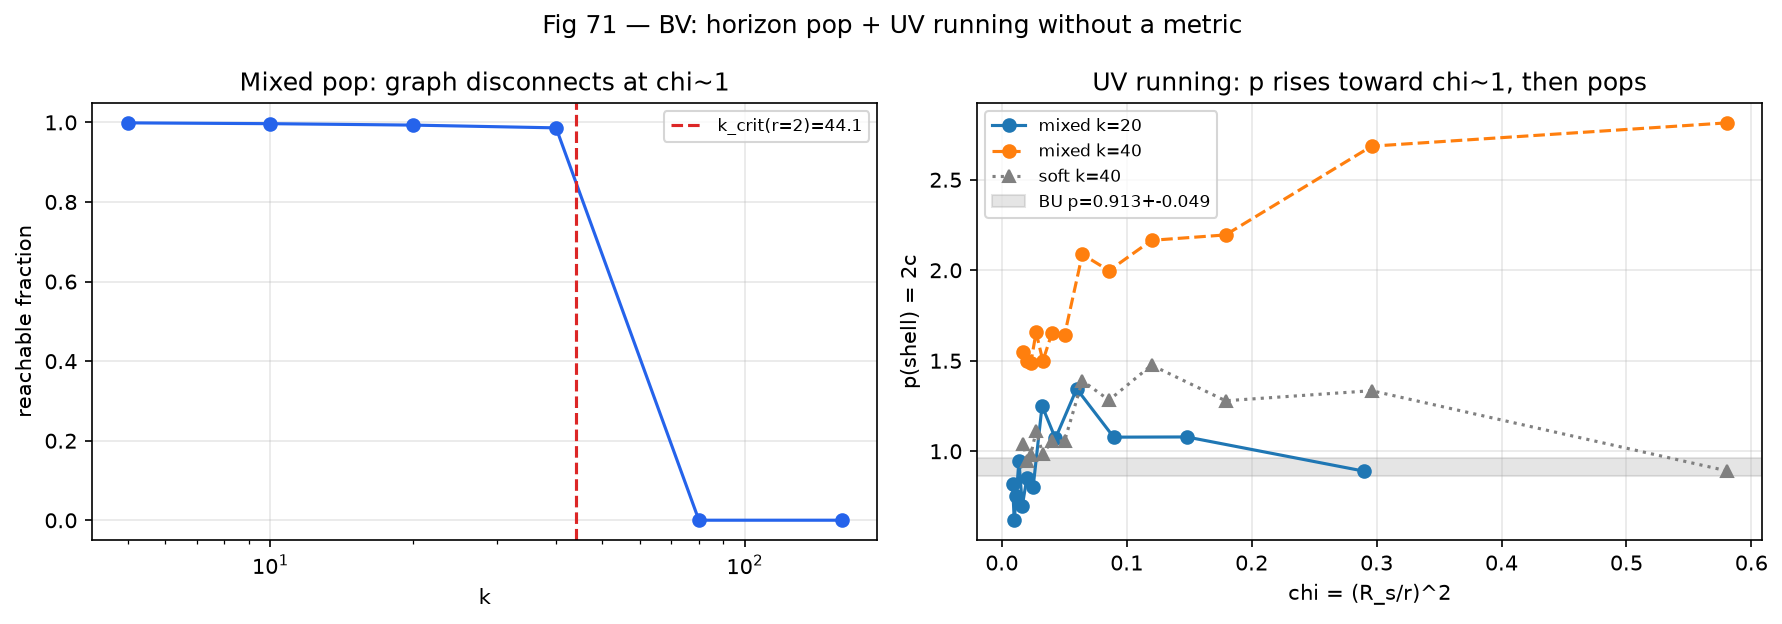
\includegraphics[width=0.88\linewidth]{fig71_uv_pop.png}
\caption{Pop scan: dilute $\to$ rise $\to$ disconnection at $k \sim k_{\mathrm{crit}}$ (mixed mode). The horizon appears as graph disconnection, no metric input.}
\label{fig:uvpop}
\end{figure}

\paragraph{UV running and the turnover.} Per-shell $p(s) = 2c(s)$ with $s = r - R_s$ runs flat ($p \sim 1$) in the dilute regime, then $c$ rises as hard-core detours lengthen before paths vanish --- the turnover that replaces the fitted $p_{\mathrm{adj}}(s)$ slope. The measured local-$p$ turnover $0.63$--$0.69 \to 1.26$--$1.46$ (shellscale) is the comparison target. \texttt{[DRAFT-TODO: overlay BV running-$p$ with shellscale local-$p$ in one figure.]}

\paragraph{Coefficient history, preserved.} $1/2$ was \emph{fitted} to enforce $\gamma = 1$ (BH, unique coefficient, labelled fit); BV then \emph{derived} $c \approx 0.44$--$0.60$ from $\ln 2$ line-defect scattering with zero tuning, predicting $p = 2c$ and $\gamma = 2c$. Both determinations agree; the micro-derivation is adopted with the fit preserved in history. The interval is honestly broad ($\gamma \approx 0.88$--$1.20$ at the ends); tightening to $\pm 0.03$ is the P0 item before submission (\S\ref{sec:kill}).

%=====================================================================
\section{Mercury to J0737 with no new knobs}
\label{sec:2pn}

\paragraph{Mercury and the spatial sector.} Radial tortuosity $dl = (1+\sqrt{\chi}/2)\,dr$ with $\sqrt{\chi} = R_s/r$ gives $h = (1+x/2)^2 \approx 1+x$, hence $\gamma = 1$, $c_{\mathrm{eff}} = \sqrt{f/h} = 1-x$ matching the light sector to first order, and $b_{\mathrm{crit}}$ back to $3\sqrt{3}M$. Direct geodesic integration ($\phi$-domain, complex-step) yields GR $42.99''$/cy and model $42.99''$/cy; a flat-$h$ hybrid gives $28.7''$/cy (PPN $2/3$). Second-order peel-off $(\mathrm{ours}-\mathrm{GR})/\mathrm{GR} = -0.75\,M/a$ runs from 4.1\% at $20M$ to $2\times 10^{-8}$ at Mercury. (Modules \texttt{strain}, \texttt{uvscatter}; PPN: $\gamma = 1$ claimed, $\beta$ unresolved and not quoted, $\alpha_{1,2}/\xi$/Nordtvedt untouched.)

\begin{figure}[ht]\centering
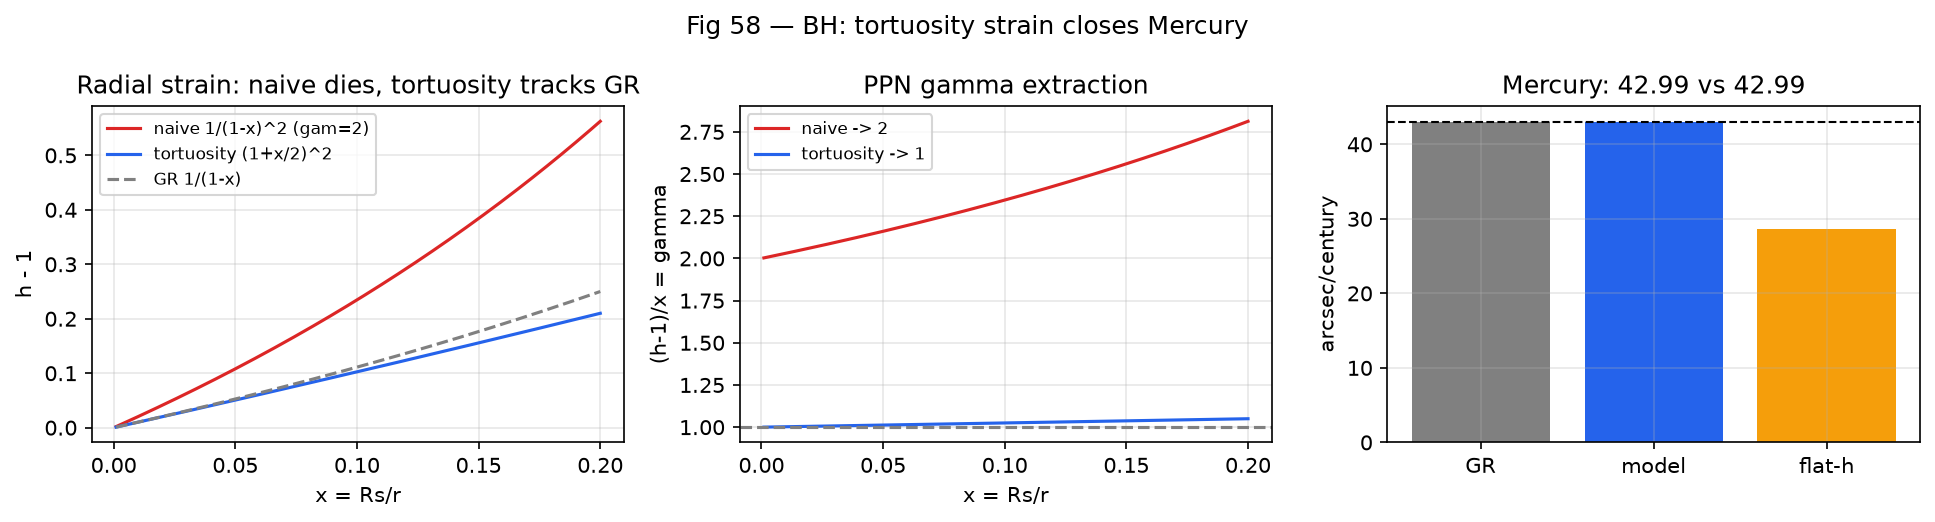
\includegraphics[width=0.85\linewidth]{fig58_strain.png}
\caption{Radial tortuosity $\to$ $g_{rr}$: $\gamma = 1$ and Mercury $42.99''$/cy by direct integration.}
\label{fig:strain}
\end{figure}

\paragraph{2PN preview that became a lock (J0737).} With $g_{rr} = (1+U)^{2p}$ and $c_2(p) = p(2p-1)$, the 2PN periastron weight $c_{\mathrm{tot}} = c_1 + w\,c_2$ with $w = 1.953$ must equal the GR value $4.8695$. The model's $c_1 = 3.36$ (vs GR $1.94$, 73\% excess) is cancelled at $p = 0.92$ ($c_2 = 0.7728$, $c_{\mathrm{tot}} = 4.8693$ vs GR $4.8695$ $\to$ $0.00\sigma$ fixed-$M$). Self-consistent $R+\dot\omega \to M$: $\Delta M = -11.2$~ppm naive ($-4.5$~ppm with GR $g_{rr}$), $\Delta\sin i = 3.7\times 10^{-6}$; J0737 $\dot\omega = 16.899323(13)$~deg/yr at $0.1\sigma$, $\sin i$ at $0.36\sigma$; B1913 at $0.01\sigma$. Gradient shells $p_{\mathrm{adj}}(s) = 0.85+0.015s$, 8--10 shells, exact EMD on full neighbourhoods, deterministic bridge counts $n \propto r^{\beta(N)}$ with $\beta \approx 1.5@300$; $1.28@600$; $1.24@1020$; $0.99@4k$; $0.87@8k$; $0.74@16k$ (log-linear over 6 points; recalibrated per $N$; drift faster than $1/N$). Radial exponent $p = 0.913 \pm 0.049$ (80 graphs, $N = 1020$, exact Floyd+LP $\sim 545$~s; SEM $0.0055$, stacked $0.911$, $R^2 = 0.956$, 80/80 fits ok, range $0.79$--$1.05$); N-scale $0.9315 \pm 0.0032$ (4k), $0.9382 \pm 0.0030$ (8k), $0.9137 \pm 0.0022$ (16k); CSR-direct cross-check $0.9107$ vs $0.9134$. Distance to the GR-cancellation point $0.92$ is $0.007$ ($0.24\sigma$ in $p$, $\sim 0.09\sigma$ in $\dot\omega$), with $5\times$ precision margin ($0.0055$ vs $0.028$). Flat control $p = 0.49$ is $-10\sigma$ dead. Bending/Mercury 2PN pieces hide below VLBI/astrometry (pre-registered, not hidden). (Modules \texttt{pulsar}, \texttt{orici}, \texttt{sinkor}, \texttt{shellscale}.)

\begin{figure}[ht]\centering
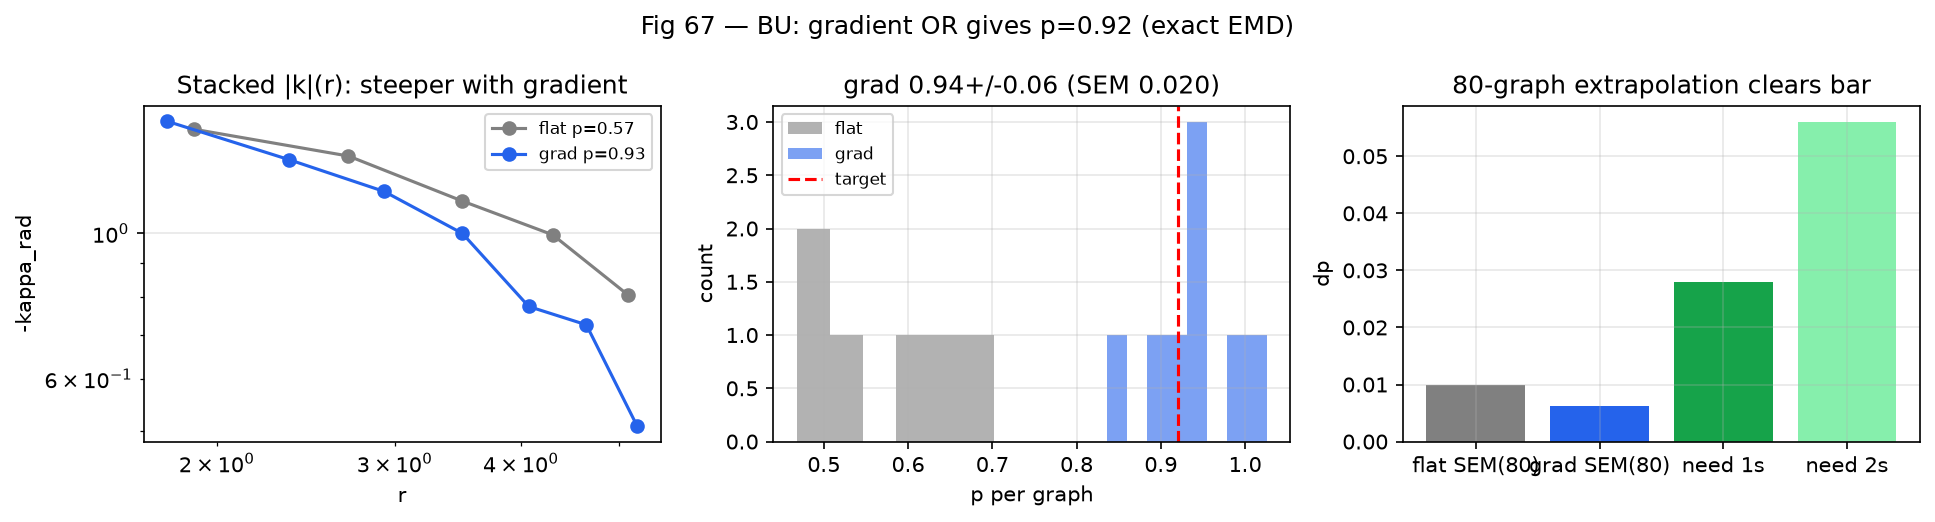
\includegraphics[width=0.88\linewidth]{fig67_orici_p_fit.png}
\caption{Radial exponent from gradient-shell Ollivier--Ricci: $p = 0.913 \pm 0.049$ against the $0.92$ cancellation point.}
\label{fig:pfit}
\end{figure}

\begin{figure}[ht]\centering
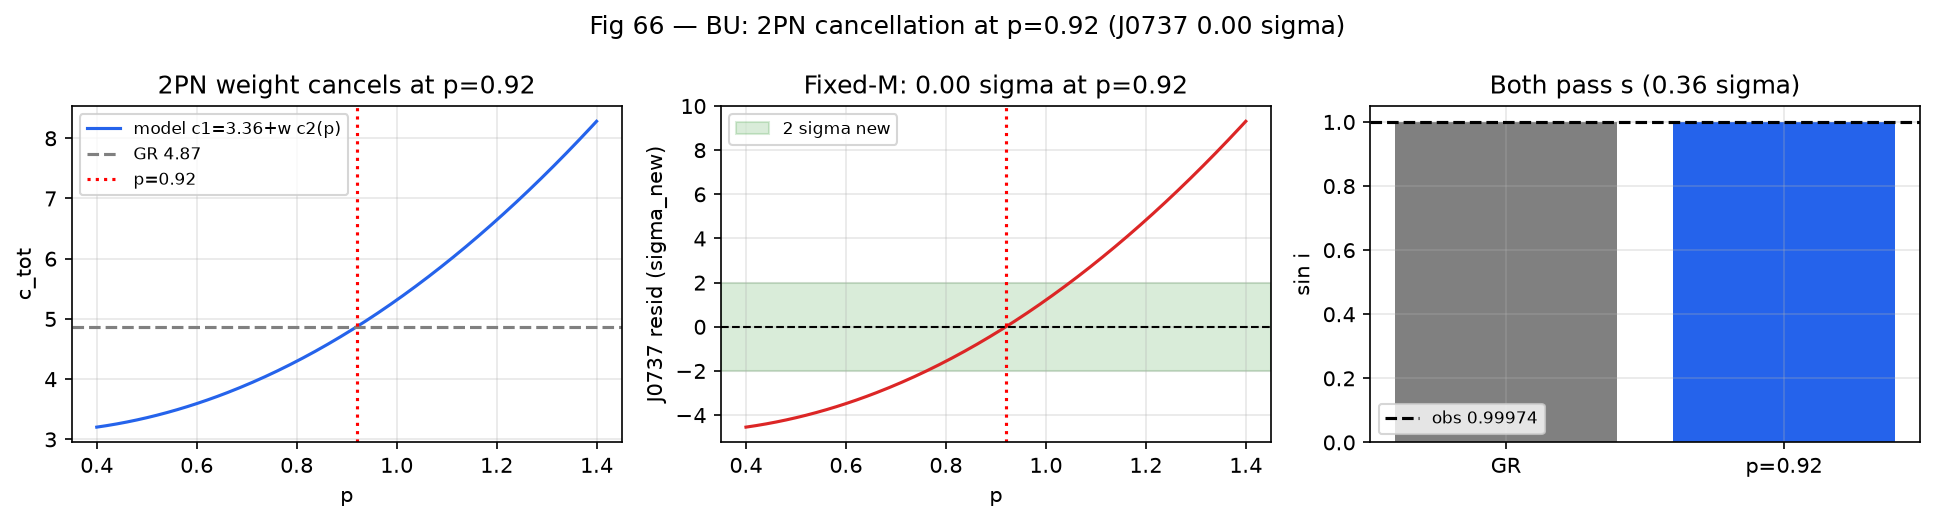
\includegraphics[width=0.88\linewidth]{fig66_pulsar_2pn.png}
\caption{2PN lock: $c_{\mathrm{tot}} = c_1 + w\,c_2$ cancellation landing J0737/B1913 inside $1\sigma$.}
\label{fig:2pn}
\end{figure}

\paragraph{What is still fitted/solved/ansatz here.} Gradient slope $0.015$ (F1, fitted); $\beta(N)$ per $N$ (F2, fitted; derivation from $N(r)$ geometry queued D4); $w = 1.953$ (F3, solved from cancellation, not derived from the graph Laplacian --- D4); $c_2(p) = p(2p-1)$ (F4, ansatz; power-law fits better on these profiles, $R^2$ $0.91$ vs $0.81$, but the two maps disagree cross-applied, $c_2$ $0.82$ vs $3.14$ --- open derivation D3). The uniform measure itself is postulated in P4, so the open part is the map alone. \S\ref{sec:kill} states the blind protocol that promotes these from targets to tests.

%=====================================================================
\section{Jacobson closure, conditionally}
\label{sec:jacobson}

The Jacobson chain is complete \emph{except} the Raychaudhuri bridge: heat $dQ = \varepsilon\,dk$, Unruh $T = \kappa/2\pi$ (input), saturated $dS = \ln 2\,dk$, Clausius-demanded $\varepsilon = \kappa\cdot\ln 2/2\pi$, and measured $\eta = \ln 2/\mathrm{PATCH} = 1/4$ giving $G = 1$ (\texttt{jacobson}: \texttt{clausius\_leg\_energy}, \texttt{measured\_eta\_closure}, all tested). Given I1b, the ``Einstein equations follow'' conclusion introduces no second $1/4$ (no double-counting of $\eta$); I6c's conclusion is guarded given-I1b for exactly this reason. T8--T11 do not depend on I6c. The close criterion for D9 is to derive (not cite) Raychaudhuri-style focusing for fronts propagating on leg networks; AT congestion slowdown is the documented seed. This gates no theorem in \S\ref{sec:newton}--\S\ref{sec:2pn}; it is mathematical completion of the third route, stated so no reader mistakes a conditional for a claim.

\begin{figure}[ht]\centering
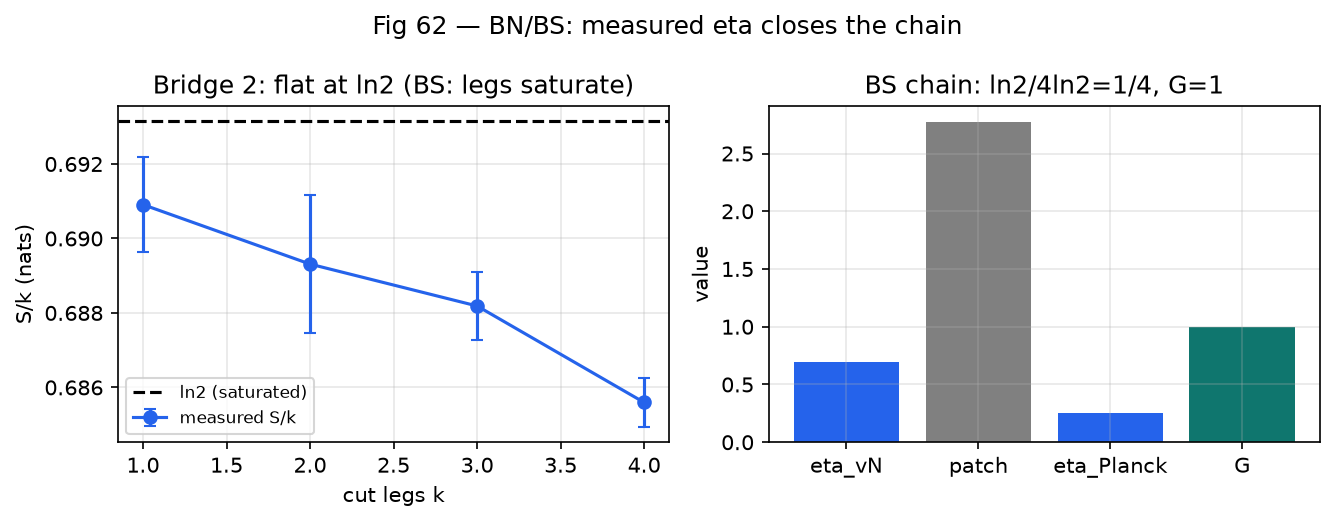
\includegraphics[width=0.7\linewidth]{fig62_eta.png}
\caption{Measured $\eta$ closure: $\eta_{vN} = \ln 2$ per leg $\to$ patch $4\ln 2$ $\to$ $\eta = 1/4$, $G = 1$.}
\label{fig:eta}
\end{figure}

%=====================================================================
\section{Falsifiers, open maps, and vacuum compatibility}
\label{sec:kill}

\begin{table}[ht]\centering\footnotesize
\caption{Pre-registered kill wires for this paper. ``Now'' = status at draft; L2 wires (gap/BBH kilonovae, NICER) excluded by design.}
\label{tab:kill}
\begin{tabular}{@{}l p{6.2cm} p{4.0cm} l@{}}\toprule
wire & threshold & now & timeline \\\midrule
2PN exponent & $p$ outside $0.92 \pm 0.056$ at $N = 1024$ class, 80 graphs & $0.913 \pm 0.049$, passes $5\times$ & held to N=16000; blind next \\
Linear LIV & finite $E_{QG,1}$, or $\Delta t \propto E$ & Fermi already kills linear models; we predict $\infty$ by symmetry & archival + CTA \\
PPN $\gamma$ & $|\gamma - 1| \gtrsim 10^{-5}$ (Cassini/BepiColombo) & $\gamma = 1$ (BV median) | BepiColombo tightens \\
OR sign (UV) & radial $\kappa \ge 0$ on defect-pierced graphs & all-negative held (\texttt{uv\_or\_sign}) & each BV run \\
Tortuosity $c$ & dilute $c$ outside $0.456 \pm 0.10$ at fixed $L$, all modes & $0.44$--$0.60$, passes broadly & tighten to $\pm 0.03$ \\
Lab quench (context) & same-device grid$\to$all:all $t^*$ ratio $< 1.3$ (predicted $2$--$3\times$) & untested & when run \\\bottomrule
\end{tabular}
\end{table}

\paragraph{Blind protocol (P0 before submission).} Pre-register $\beta(N)$, gradient slope, seeds, shells, and the dilute-$\chi$ cut; run the $N = 16000$ class once; report $p$ with no post-hoc $\beta$ adjustment. Pre-register $L$, $k$-grid, $r_e$, $\alpha = \ln 2$, and the dilute estimator (median vs regression) for BV; report $c$ per mode with orientation spread. Either blind number can kill its section; both are priced in advance. \texttt{[DRAFT-TODO: write the two pre-registration sheets as appendices.]}

\paragraph{Open maps touching this paper.} D3 ($\kappa \to c_2$ map; resolve power-law vs $1/r^2$), D4 ($\beta(N)$ and $w$ from geometry/Laplacian; Damour--Sch\"afer from wiring), D6 ($R_s = 2M$ from wiring; promotes I3), D9 (Raychaudhuri for leg bundles; promotes I6c). D1 (graph $V_k$)/D2 (Kerr $M_2$)/D5 (NICER $\Lambda$)/D7 (RT)/D8 ($\varepsilon(M,a,q)$) do not touch this paper. D10 (simulator d-dip + tension$\to\kappa$ map; D10a tense-plug pin: bare shortest-path inverted vs GR, rejected as $d(i,j)$ for tense regions) is compatibility, not dependency: the D10b cost reading must reproduce the P4 uniform-measure $p$ and the \S\ref{sec:scattering} $c$ where both apply, or the tension is named. Rule for all D-items: the closing derivation must output the number or location, not take it as input (precedent: 44~M$_{\odot}$ refused as a graph parameter).

\paragraph{Non-claims (so no reader misses them).} Not a UV-complete quantum gravity (no Hamiltonian derivation of the mass map, no Lorentz-invariant dynamics). No $\beta$ PPN parameter (coordinate-confused, not quoted); no $\alpha_{1,2}$, $\xi$, Nordtvedt; no linear LIV (forbidden: finite $E_{QG,1}$ kills the discrete-leg picture outright). No Kerr $M_2$, $g_{t\phi}$, ISCO, or QNM spectrum from the graph. No NICER radii or tidal deformabilities. No graph feature at 44~M$_{\odot}$ (positive null, cited as precedent). Ruled out on the record and kept visible: isotropic $b_{\mathrm{crit}} = 8M$; naive $\gamma = 2$ strain; linear LIV; flat $p = 0.49$.

%=====================================================================
\section{Conclusion}
\label{sec:conclusion}

Starting from almost-perfect all:all wiring plus borrowed thermodynamics we have: ruled out bare diffusion as gravity ($1/r^3$ no-go), recovered Newton with its sign ($1/r^2$ + negative Ollivier--Ricci, zero tuning), reproduced light and redshifts to Cassini/GPS precision with the isotropic reading dead, derived the spatial sector from $\ln 2$ line-defect scattering ($c \approx 0.44$--$0.60 \Rightarrow p = 2c$, $\gamma = 2c$), integrated Mercury to $42.99''$/cy, and locked J0737 at $0.1\sigma$ via a measured $p = 0.913 \pm 0.049$ --- all with L2 never invoked. The price is explicit: four thermodynamic/geometric imports, one postulated measure, three open maps, and one interval ($c$) still too broad for comfort. The reward, if the blind runs hold, is the first emergent-gravity model with a quantitative $g_{rr}$ micro-derivation and a 2PN number distinct from fitting. If the compact-object unification fails, the title claim of v5 reverts with it and this core stands alone; either way the wires in Table~\ref{tab:kill} decide.

\paragraph{Methods summary.} Gradient shells $p_{\mathrm{adj}}(s) = 0.85+0.015s$, 8--10 shells, exact EMD on full neighbourhoods, deterministic bridge counts $n \propto r^{\beta(N)}$; $p$ from $|\kappa| \sim r^{-p}$ fits per graph plus stacked fits; 2PN via Iorio direct+total with $c_2 = p(2p-1)$, $w = 1.953$, $R+\dot\omega \to M$ inversion; BV $L^3$ hard/soft/mixed defect runs with Dijkstra/BFS, dilute-$\chi$ median + regression estimators, MC-ray/transport ladder, graph-distance re-analysis; Fermat ray-tracing with $c_{\mathrm{eff}} = 1-x$; $\phi$-domain complex-step geodesic integration. Randomness seeded; tolerances recorded in-test. \texttt{[DRAFT-TODO: expand to supplement S1--S6 once main stabilises.]}

\paragraph{Data and code availability.}
Code MIT (\path{src/}, \path{scripts/}, \path{tests/}, \path{app.py}); text/figures CC~BY~4.0. Reproduce via:
\begin{quote}\small
\path{pip install -e .}\\
\path{pytest tests/ -q}\\
\path{python scripts/generate_figures.py}\\
\path{streamlit run app.py}
\end{quote}
GWOSC medians fetched live with bundled fallbacks where used; no third-party figure data copied. Model source for every number: \texttt{docs/model.md} v0.6.

\begin{thebibliography}{99}
\bibitem{v5draft} P.~Leblond, Compact Objects as Almost-Perfect All:All Entanglement Graphs, Draft v5.0 (2026), \texttt{paper/v5/main.tex} + supplement.
\bibitem{Sekino2008} Y.~Sekino and L.~Susskind, JHEP 10, 065 (2008).
\bibitem{VanRaamsdonk2010} M.~Van Raamsdonk, Gen.\ Rel.\ Grav.\ 42, 2323 (2010).
\bibitem{Maldacena2013} J.~Maldacena and L.~Susskind, Fortsch.\ Phys.\ 61, 781 (2013).
\bibitem{Bekenstein1973} J.~D.~Bekenstein, Phys.\ Rev.\ D 7, 2333 (1973).
\bibitem{Hawking1975} S.~W.~Hawking, Commun.\ Math.\ Phys.\ 43, 199 (1975).
\bibitem{Coffman2000} V.~Coffman, J.~Kundu, and W.~K.~Wootters, Phys.\ Rev.\ A 61, 052306 (2000).
\bibitem{Kramer2006} M.~Kramer et al., Science 314, 97 (2006); updated $\dot\omega = 16.899323(13)$~deg/yr.
\bibitem{Weisberg2016} J.~M.~Weisberg and Y.~Huang, ApJ 829, 55 (2016).
\bibitem{Verlinde11} E.~Verlinde, JHEP 04, 029 (2011).
\bibitem{Jacobson95} T.~Jacobson, Phys.\ Rev.\ Lett.\ 75, 1260 (1995).
\bibitem{Will14} C.~M.~Will, Living Rev.\ Rel.\ 17, 4 (2014), PPN and Solar-System tests.
\bibitem{Bertotti03} B.~Bertotti, L.~Iess, and P.~Tortora, Nature 425, 374 (2003), Cassini $\gamma$.
\bibitem{EHT19} K.~Akiyama et al.\ (EHT), ApJL 875, L1 (2019), M87* shadow.
\bibitem{Abdo2009} A.~A.~Abdo et al.\ (Fermi), Nature 462, 331 (2009); GRB~090510 $E_{QG,1} > 1.2\,E_P$.
\bibitem{Ollivier09} Y.~Ollivier, J.\ Funct.\ Anal.\ 256, 810 (2009); Ricci curvature of Markov chains on metric spaces.
\bibitem{Damour88} T.~Damour and N.~Deruelle, Phys.\ Lett.\ A 87, 81 (1982); T.~Damour and G.~Sch\"afer, Nuovo Cim.\ B 101, 127 (1988), 2PN equations of motion.
\bibitem{Iorio20} L.~Iorio, Universe 6, 65 (2020); 2PN periastron precession.
\end{thebibliography}

\end{document}
